\section{Experimental Validation} \label{sc:experimental-validation}
In order to do a qualitative and quantitative analysis of the algorithms presented in Section \ref{sc:state-of-the-art}, a set of trials based on synthetic images was set up. The carried evaluation is twofold: (1) the algorithms were evaluated using synthetic images which were degenerated with a known type of noise and specific parameters for them; (2) we tested the different denoising techniques on retinopathy images. The complexity of denoising these images is that the kind of noise and its parameter are not known. Therefore, some noisy parameters have to be estimated.

\subsection{Synthetic images} \label{sc:experimental_sythetic}
When talking about synthetic images, one makes reference to those in which the level of noise is low.  The interest of using this kind of images for testing is that they have some characteristics related, for instance, to the content of high frequencies or low frequencies. Degenerated versions of these images can be used to evaluate the performance of denoising algorithms since the originals are known. To make the synthetic images, the three images shown in Fig. \ref{fig:setup_synthetic_originals} were noised in purpose. Cameraman image is characterised by having low frequencies, Lena image has intermediate frequencies and baboon image is composed by high frequencies. Therefore, using this images as a base of the synthetic images will give a proper analysis expanding the vast majority of the frequency range.

\begin{figure}[H]
  \centering
 \begin{tabular}{c c c c c}
     \begin{varwidth}{0.5\linewidth}
       \subfigure{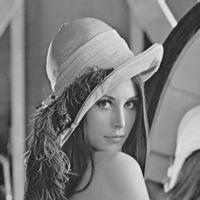
\includegraphics[width=16mm]{Figures/setup_synthetic_images/lena.jpg}}
     \end{varwidth}
     \begin{varwidth}{0.5\linewidth}
       \subfigure{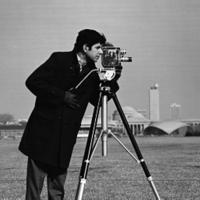
\includegraphics[width=16mm]{Figures/setup_synthetic_images/cameraman.jpg}}
     \end{varwidth}
     \begin{varwidth}{0.5\linewidth}
       \subfigure{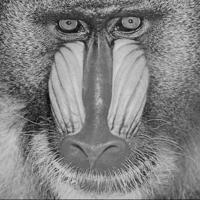
\includegraphics[width=16mm]{Figures/setup_synthetic_images/baboon.jpg}}
     \end{varwidth}
 \end{tabular}
  \caption{Original images. From left to right: Lena, cameraman and baboon.} 
  \label{fig:setup_synthetic_originals}
\end{figure}

Each one of these images was corrupted with 5 different types of noise: Gaussian, Rician, uniform, salt and pepper and speckle noise. While the first four types of noise are additive, the last one is multiplicative. Specifically, the characteristic parameters of each kind of noise are represented in Table \ref{tb:noising_parameters}.

\begin{table}[H]
    \centering
    \caption{Characteristics of the different types of noise.}
    \begin{tabular}{|c|c|}
    \hline
    \textbf{Type of noise} & \textbf{Characteristics} \\ \hline
    Gaussian & $\mu$=0 , $\sigma$=0.1 \\ \hline
    Rician & $\mu$=0.05 , $\sigma$=0.1 \\ \hline
    Uniform & $\mu$=0 , $\sigma$=0.1 \\ \hline
    Salt and Pepper & 5\% salt , 5\% pepper \\ \hline
    Speckle & $\mu$=0 , $\sigma$=0.04 \\ \hline
    \end{tabular}
    \label{tb:noising_parameters}
\end{table}

After applying the described noises in the original images seen in Fig. \ref{fig:setup_synthetic_originals}, the obtained noisy images are the ones shown in Fig. \ref{fig:setup_synthetic_noised}.

\begin{figure}[H]
  \centering
 \begin{tabular}{c c c c c}
     \begin{varwidth}{0.5\linewidth}
       \subfigure{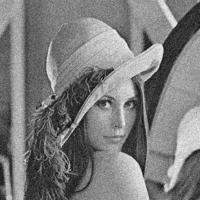
\includegraphics[width=16mm]{Figures/setup_synthetic_images/lena_nor.jpg}}\\
       \subfigure{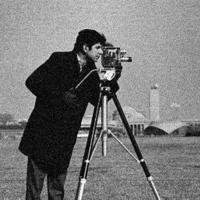
\includegraphics[width=16mm]{Figures/setup_synthetic_images/cameraman_nor.jpg}}\\
       \subfigure{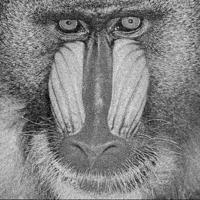
\includegraphics[width=16mm]{Figures/setup_synthetic_images/baboon_nor.jpg}}
     \end{varwidth}
     \begin{varwidth}{0.5\linewidth}
       \subfigure{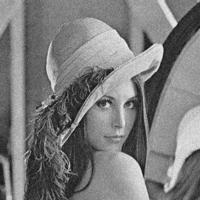
\includegraphics[width=16mm]{Figures/setup_synthetic_images/lena_ric.jpg}}\\
       \subfigure{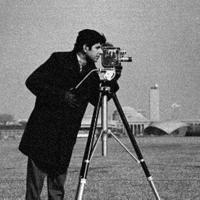
\includegraphics[width=16mm]{Figures/setup_synthetic_images/cameraman_ric.jpg}}\\
       \subfigure{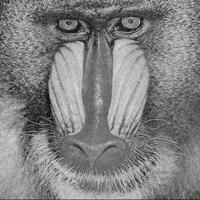
\includegraphics[width=16mm]{Figures/setup_synthetic_images/baboon_ric.jpg}}
     \end{varwidth}
     \begin{varwidth}{0.5\linewidth}
       \subfigure{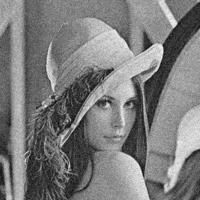
\includegraphics[width=16mm]{Figures/setup_synthetic_images/lena_uni.jpg}}\\
       \subfigure{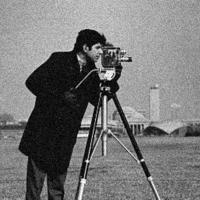
\includegraphics[width=16mm]{Figures/setup_synthetic_images/cameraman_uni.jpg}}\\
       \subfigure{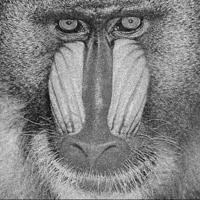
\includegraphics[width=16mm]{Figures/setup_synthetic_images/baboon_uni.jpg}}
     \end{varwidth}
     \begin{varwidth}{0.5\linewidth}
       \subfigure{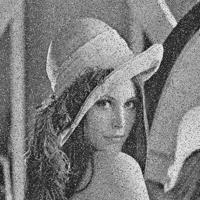
\includegraphics[width=16mm]{Figures/setup_synthetic_images/lena_sp.jpg}}\\
       \subfigure{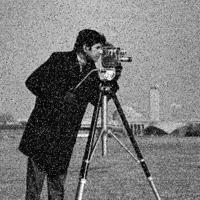
\includegraphics[width=16mm]{Figures/setup_synthetic_images/cameraman_sp.jpg}}\\
       \subfigure{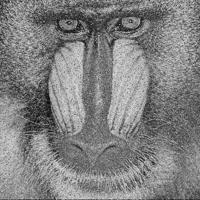
\includegraphics[width=16mm]{Figures/setup_synthetic_images/baboon_sp.jpg}}
     \end{varwidth}
     \begin{varwidth}{0.5\linewidth}
       \subfigure{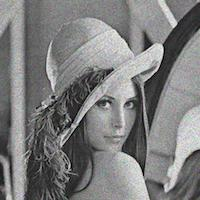
\includegraphics[width=16mm]{Figures/setup_synthetic_images/lena_spec.jpg}}\\
       \subfigure{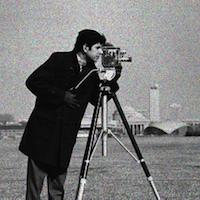
\includegraphics[width=16mm]{Figures/setup_synthetic_images/cameraman_spec.jpg}}\\
       \subfigure{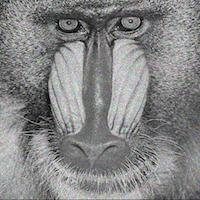
\includegraphics[width=16mm]{Figures/setup_synthetic_images/baboon_spec.jpg}}
     \end{varwidth}
 \end{tabular}
  \caption{Noised images. From left to right: additive Gaussian, additive Rician, additive uniform, additive salt and pepper and multiplicative speckle noise, respectively.} 
  \label{fig:setup_synthetic_noised}
\end{figure}

For visualization purposes, all the images shown in Section \ref{sc:results} will be shown in a colormap format. As can be seen in Fig. \ref{fig:setup_synthetic_noised_color}, the noise added to the images in Fig. \ref{fig:setup_synthetic_noised} can be better with this color visualization. 

\begin{figure}[H]
  \centering
 \begin{tabular}{c c c c c}
     \begin{varwidth}{0.5\linewidth}
       \subfigure{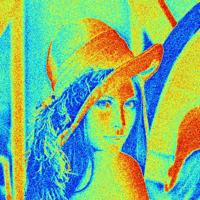
\includegraphics[width=16mm]{Figures/setup_synthetic_images/color_lena_nor.jpg}}\\
       \subfigure{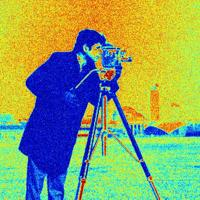
\includegraphics[width=16mm]{Figures/setup_synthetic_images/color_cameraman_nor.jpg}}\\
       \subfigure{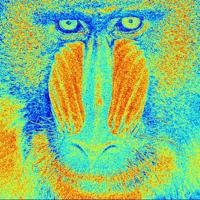
\includegraphics[width=16mm]{Figures/setup_synthetic_images/color_baboon_nor.jpg}}
     \end{varwidth}
     \begin{varwidth}{0.5\linewidth}
       \subfigure{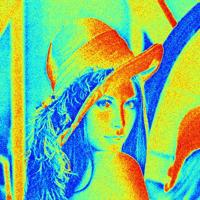
\includegraphics[width=16mm]{Figures/setup_synthetic_images/color_lena_ric.jpg}}\\
       \subfigure{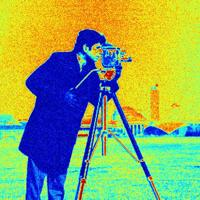
\includegraphics[width=16mm]{Figures/setup_synthetic_images/color_cameraman_ric.jpg}}\\
       \subfigure{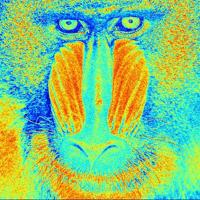
\includegraphics[width=16mm]{Figures/setup_synthetic_images/color_baboon_ric.jpg}}
     \end{varwidth}
     \begin{varwidth}{0.5\linewidth}
       \subfigure{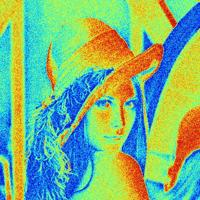
\includegraphics[width=16mm]{Figures/setup_synthetic_images/color_lena_uni.jpg}}\\
       \subfigure{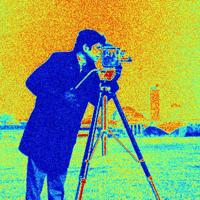
\includegraphics[width=16mm]{Figures/setup_synthetic_images/color_cameraman_uni.jpg}}\\
       \subfigure{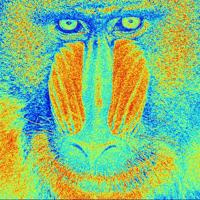
\includegraphics[width=16mm]{Figures/setup_synthetic_images/color_baboon_uni.jpg}}
     \end{varwidth}
     \begin{varwidth}{0.5\linewidth}
       \subfigure{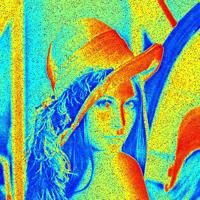
\includegraphics[width=16mm]{Figures/setup_synthetic_images/color_lena_sp.jpg}}\\
       \subfigure{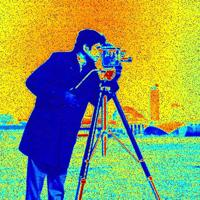
\includegraphics[width=16mm]{Figures/setup_synthetic_images/color_cameraman_sp.jpg}}\\
       \subfigure{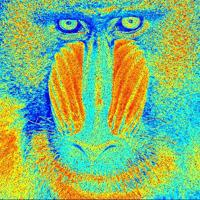
\includegraphics[width=16mm]{Figures/setup_synthetic_images/color_baboon_sp.jpg}}
     \end{varwidth}
     \begin{varwidth}{0.5\linewidth}
       \subfigure{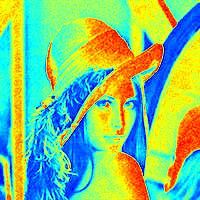
\includegraphics[width=16mm]{Figures/setup_synthetic_images/color_lena_spec.jpg}}\\
       \subfigure{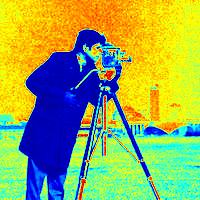
\includegraphics[width=16mm]{Figures/setup_synthetic_images/color_cameraman_spec.jpg}}\\
       \subfigure{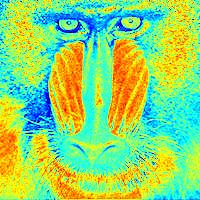
\includegraphics[width=16mm]{Figures/setup_synthetic_images/color_baboon_spec.jpg}}
     \end{varwidth}
 \end{tabular}
  \caption{Noised images represented in a colormap format. From left to right: additive Gaussian, additive Rician, additive uniform, additive salt and pepper and multiplicative speckle noise, respectively.} 
  \label{fig:setup_synthetic_noised_color}
\end{figure}

\subsection{Retinopathy images}
In the previous section, we presented an evaluation based on noising synthetic images in which the noise characteristics were known in advance. However, these parameters are usually not given in real-life scenarios. To evaluate the algorithm under this kind of conditions, we consider Spatial-Domain Optical coherence tomography (SD-OCT) images. The evaluation using these images consists of the following steps. First, a volume of OCT is taken and processed using the different considered algorithms. For this task, we consider the dataset provided by the University of Girona \cite{udg}. Second, the noise is estimated and the determined value is used as input for the K-SVD algorithm. 

\begin{figure}[H]
  \centering
      \subfigure{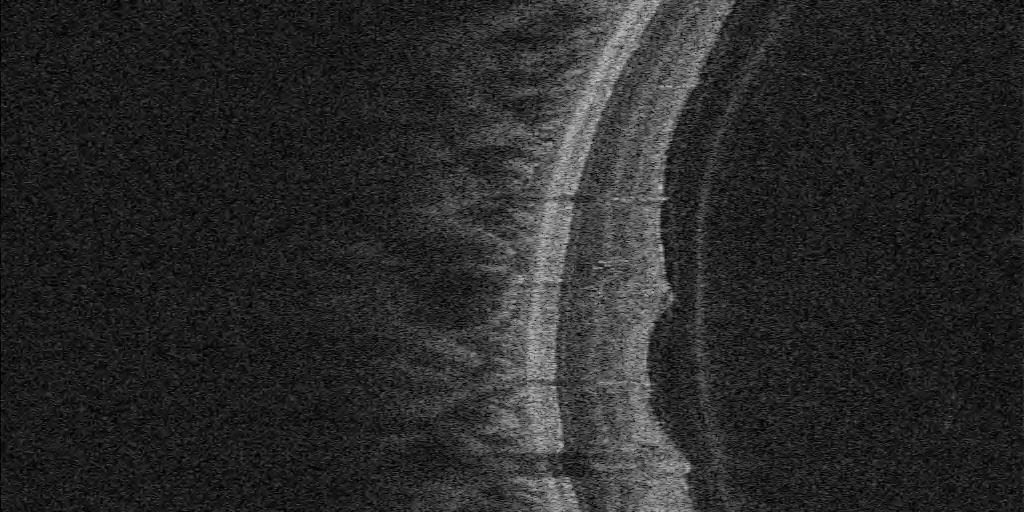
\includegraphics[width=80mm]{Figures/setup_retinopathy/original_P741009OS.jpg}}
  \caption{Retinopathy image.} 
  \label{fig:setup_retinopathy_image_setup}
\end{figure}

The goal of denoising retinopathy images is to obtain a better segmentation of the different retinopathy layers. For this, the resulting denoised images are segmented using the tool called OCT Explorer developed by the University of Iowa \cite{iowa}. Finally, the outcome of the segmentation is compared against the segmentation of the noisy retinopathy volume, which can be seen in Fig. \ref{fig:setup_retinopathy_segmentation_setup}.

\begin{figure}[H]
  \centering
      \subfigure{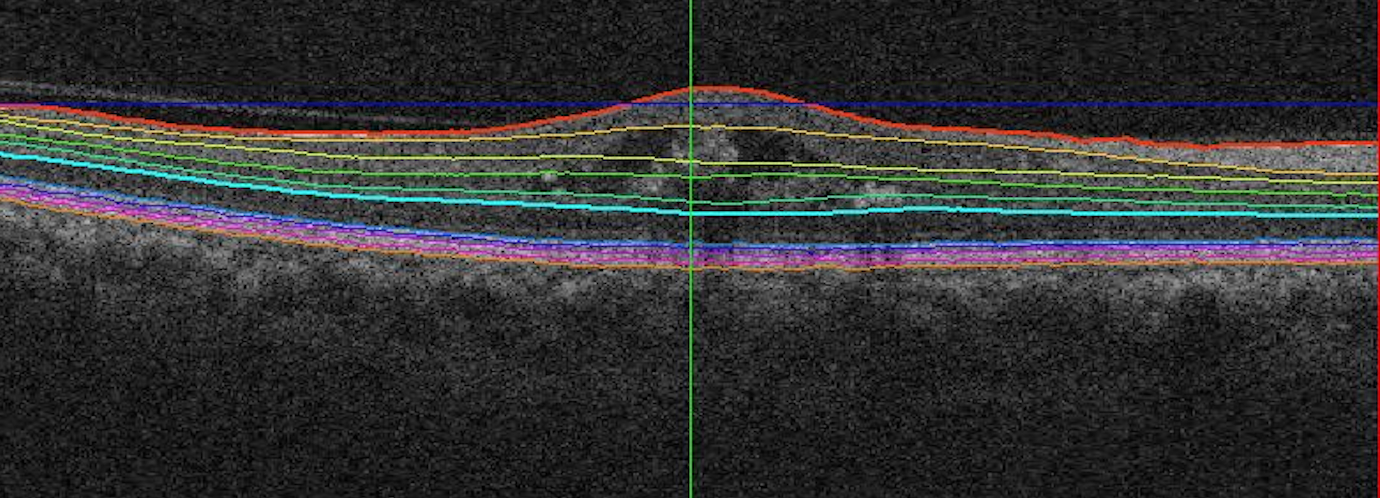
\includegraphics[width=80mm]{Figures/setup_retinopathy/original_segmentation.jpg}}
  \caption{Segmentation of a noisy retinopathy volume.} 
  \label{fig:setup_retinopathy_segmentation_setup}
\end{figure}

The output segmentation of the noisy volume shows up all the 11 existing layers of the retina. Since there is not any ground-truth to check the accuracy of the resulting segmentations, only the number of obtained layers and a visual analysis can be given in the following analysis.  